\documentclass[dvipdfmx,18pt]{jsarticle}
\usepackage{graphics}
\usepackage{amsmath}
\usepackage{amssymb}
\usepackage{amsthm}
\usepackage{mathtools}
\usepackage{ascmac}
\usepackage{bm}
\usepackage{url}
\usepackage{txfonts}
\usepackage{color}
\usepackage{tikz}
\usetikzlibrary{calc}
\usetikzlibrary{intersections}

\begin{document}
    \section*{初めに}
    中学数学の中でのやや面倒な単元である濃度と密度について扱う.この2つは根元のところで同じなので,同時に理解したい.この資料は中学生向けではある.しかし,読みにくい場合は両親の助けを借りるように.

    さて,早速だがこの資料で一番大事なテーマをここで示しておく.それは

    {\centering 一部分がわかれば全体の様子がわかる\\}
    というものだ.
    これは科学(理系の勉強)のすべてに共通する大事な発想だ.濃度・密度は一部分を知ることで全体がわかる最も簡単な例になっている.


    次の節から本題に入る.まずは濃度から扱う.

    \section{濃度}
    \subsection{同じしょっぱさ}
    食塩水の濃度を考える問題では,外すことができない大事な条件がある.問題文には書かれていないことが多い.それは,"食塩水は完全に混ざっている"という条件だ.簡単に言うと,食塩水のどの部分を飲んでも同じしょっぱさだということだ.そして,それは大きな食塩水のバケツからいくらコップに食塩水をくんできても同じものになるということでもある(図\ref{tikz_baketu_shokuensui}).

    \begin{figure}[htbp]\centering
        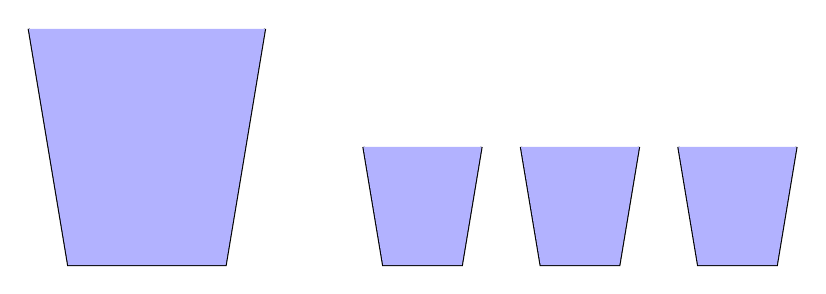
\begin{tikzpicture}\large
            \draw[thick]($2*(-.25,1.5)$)--(0,0)--($2*(1,0)$)--($2*(1.25,1.5)$);
            \fill[blue!30]($2*(-.25,1.5)$)--(0,0)--($2*(1,0)$)--($2*(1.25,1.5)$);

            \foreach \x in {4,6,8}{
                \draw[thick](\x -.25,1.5)--(\x,0)--(\x +1,0)--(\x +1.25,1.5);
                \fill[blue!30](\x -.25,1.5)--(\x,0)--(\x +1,0)--(\x +1.25,1.5);
            }

        \end{tikzpicture}
        \caption{大きなバケツから食塩水をとる}
        \label{tikz_baketu_shokuensui}
    \end{figure}
    

\end{document}
